The direct impact of a prompt or prompt strategy on model outputs, as well as the modification of LLMs' billions of parameters during re-training, are both active areas of research~\cite{liu2021pretrain,sanh2022multitask}. Recent research~\cite{xing2023prompt,white2023prompt,lian2023llmgrounded} provides some insights into effective prompt design strategies.~\citet{brown2020language} demonstrated that examples significantly enhanced GPT-3's performance across tasks such as question answering and language translation. We focus on designing effective prompts for fact-checking. Additionally, we release our prompted results as a pseudo-labeled dataset to establish a benchmark on this task.

\begin{figure*}
  \centering
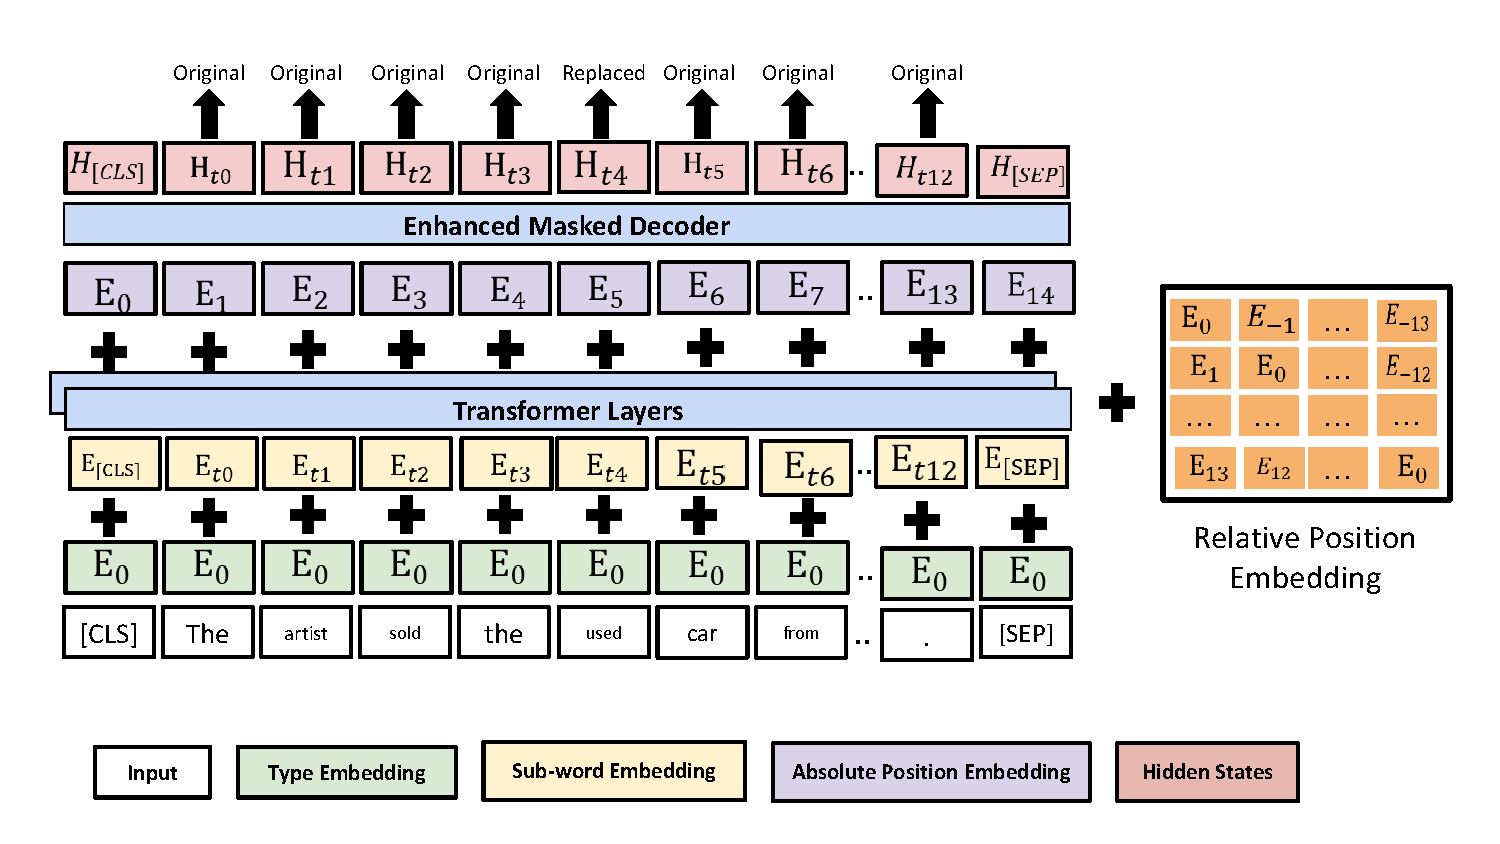
\includegraphics[width=\textwidth,height=\textwidth,keepaspectratio]{images/deberta.pdf}
  \caption{Overview of training strategy in DeBERTa V3: This figure involves passing sub-word embedding which is token embedding through several transformer layers, adding it to position embedding. It then goes through another transformer layer, followed by training using replacing token detection. The position embedding is divided into absolute and relative components. Absolute follows the original BERT, emphasizing absolute word positions. Relative, on the other hand, emphasizes relative positions. This approach highlights absolute word positions in the final layer.}
  \label{fig:deberta}
\end{figure*}